%Chapter 1 - Intro

\section{History}
The EMC effect was first discovered by its namesake the European Muon Collaboration (EMC group) in 1983. The EMC group measured the structure functions of hydrogen, deuterium, and iron. After correcting for the neutron excess, the per nucleon $F_2$ structure function ratio of iron to deuterium was calculated, as seen in Figure \ref{emc_fe}. This data showed a clear $x$ dependence, contrary to expectations.

\begin{figure}
\begin{center}
	\includegraphics[width=0.5\textwidth]{./EMC/fig/original_EMC.png}
	\caption{Results from the EMC collaboration showing a clear $x$ dependence of the per-nucleon $F_2$ structure function ratio\cite{emc_FE}}
	\label{emc_fe}
\end{center}
\end{figure}

Prior to this original measurement, nucleons were assumed to be quasi-free within the nucleus. In this understanding the nuclear $F_2$ structure function would be described as
\begin{equation}
	F_2^A = ZF_2^p + \left(A-Z\right)F_2^n.
\end{equation}
This description leads to the prediction that the per nucleon structure function ratio of any two isoscalar targets will be unity. At this time, the only other expected nuclear effect was Fermi motion. Fermi motion causes a sharp rise in the per nucleon structure function ratio at high x, but would leave the ratio largely unchanged at low x.

The original experiment did not originally set out to measure the EMC effect, rather the data was a byproduct of efforts to achieve higher luminosity. Because of this, the data had very large uncertainty on the measurement. However, the uncertainties were small enough that the anomaly could be confirmed.

Shortly after the original EMC measurement a Rochester-SLAC-MIT group analyzed previous SLAC data to confirm the phenomenon. The data analyzed not only confirmed the effect in iron, but also in aluminum. The iron data showed the EMC effect as well as the expected rise from Fermi motion at high $x$. The aluminum data showed these phenomena as well as low $x$ shadowing and anti-shadowing. \cite{bodek_Fe,bodek_Al,Norton}

\section{Further Results}

Since that time, numerous experiments have measured nuclear $F_2$ structure function data in order to better understand the nature of this anomaly. These searches have primarily focused on heavy isoscalar nuclei. The following represents a non-exhaustive presentation of these experiments.

\subsection{SLAC}
At SLAC a new experiment was set up with the explicit goal of measuring the EMC effect in a wide range of nuclei. The data cover a large kinematic range of $0.089 \le x \le 0.8$ and $2 \left(\textrm{GeV/c}\right)^2 \le Q^2 \le 15 \left(\textrm{GeV/c}\right)^2$. This data confirms the phenomenon seen by the EMC group in the $x>0.3$ region, but also sees a downturn in the ratios at low x. 

The targets studied were $^4$He, Be, C, Al, Ca, Fe, Ag, and Au. These results are shown in Figure \ref{gomez_results}. This target range allowed them to study the mass number $A$-dependence of the EMC effect. This data suggests an approximately $\ln\left(A\right)$ dependence on the strength of the EMC effect, with notable outliers of $^4$He and Be. \cite{Arnold,Gomez}

\begin{figure}[h]
\begin{center}
	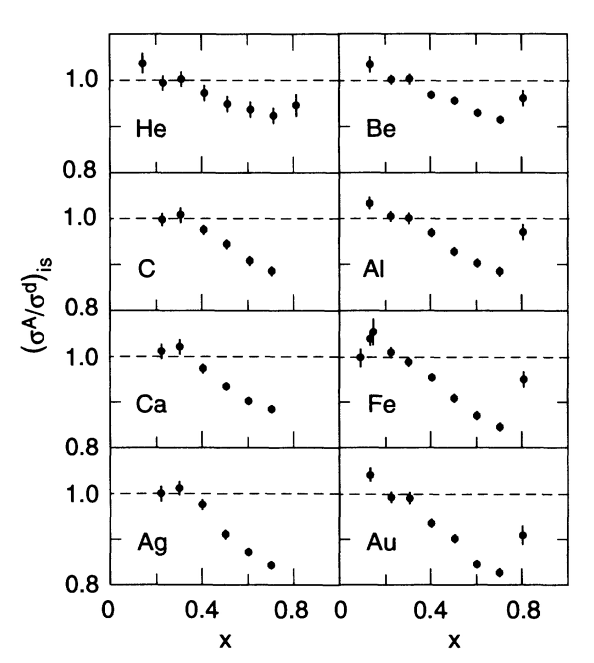
\includegraphics[width=0.5\textwidth]{./EMC/fig/gomez.png}
	\caption{Results from SLAC showing an A-dependent EMC effect\cite{Gomez}}
	\label{gomez_results}
\end{center}
\end{figure}

%\textbf{Neutrino}

\subsection{BCDMS}
The BCDMS experiment at CERN measured the N and Fe EMC ratios. The iron data is consistent with the original EMC measurement within a normalization discrepancy. The nitrogen data is consistent with the SLAC carbon data. The BCDMS results show no $Q^2$ dependence in the EMC effect. However, BCDMS does not demonstrate an $A$-dependence of the EMC effect as SLAC did.\cite{Norton} %This is potentially due to larger uncertainties on the data at high $x$.

\subsection{EMC} 
The EMC group performed three more experiments to study the EMC effect.

The first of these experiments set out to improve the systematics of the original experiment. This followup measured the EMC ratio of C, Cu, and Sn. This data agrees with the original data for $x \geq 0.08$. However, below this threshold the data sees a downturn, the shadowing region, that the original experiment did not see.\cite{ashmanEMC}

The NA28 experiment focused on studying the EMC ratio of C and Ca at low $x$. This data confirms the shadowing effect seen in the previous EMC data, the ratio drops below unity in the region of $x<0.1$. These results also shows that the shadowing region has no $Q^2$ dependence. The data overlaps well with previous measurements.

The last EMC group experiment to study the EMC effect remeasured the copper EMC ratio. To minimize systematics two 1m $^2$H targets and three Cu targets were used. These results agree with the results from the first followup and are of greater precision. %They have been combined with old data???

\subsection{NMC}
The New Muon Collaboration (NMC) continued the study of the EMC effect at CERN. Initially NMC measure the EMC ratio of Li, C, and Ca to high precision at low $x$. This data was taken with two goals: to confirm the EMC data in the shadowing region and to study the effect of nuclear size and density on the EMC ratio. The data confirms the previous EMC measurement and found a very weak $Q^2$ dependence. Lithium and carbon have approximately the same size nucleus, but different nuclear densities. Calcium and carbon have the approximately the same nuclear density, but calcium has a bigger nucleus. It was found that both of these factors play a part in the suppression of the EMC ratio in the shadowing region. Increases in nuclear size or density show an increase in the suppression of the EMC ratio due to nuclear shadowing.

NMC then set out to study the difference between the photonuclear $R$ of different targets in the region of $0.01 \leq x \leq 0.3$. The results were found, within uncertainties, to be compatible with zero. This result confirms that $\nicefrac{\sigma_A}{\sigma_D}=\nicefrac{F_2^A}{F_2^D}$.

Finally, the NMC group studied the EMC effect on Be, C, Al, Ca, Fe, Sn, and Pb. These results again confirm that there is no $Q^2$ dependence of the EMC ratio above $x=0.06$. These data agree with the SLAC result finding that the EMC effect is approximately logarithmic with $A$.\cite{NMC}

%\textbf{E665}

\subsection{HERMES}
The HERMES experiment ran at the HERA collider. This experiment collided positrons with protons to study the EMC effect on $^3$He and N. Data was taken for $0.013 \le x \le 0.65$ and $0.5 \left(\textrm{GeV/c}\right)^2 \le Q^2 \le 15 \left(\textrm{GeV/c}\right)^2$. In the $x<0.06$ region, the HERMES results differed drastically from the NMC results. Initially this was misreported as an $A$ dependence of photonuclear $R$. This reporting was later amended when it was found that the difference could be attributed to a previously unaccounted for systematic effect.

\subsection{JLab}
The E03-103 experiment ran in Hall C at Jefferson Lab. This experiment studied the EMC effect in $^3$He, $^4$He, Be, and C. The kinematics covered were $0.3 < x < 0.9$ and $3 \left(\textrm{GeV/c}\right)^2 < Q^2 < 6 \left(\textrm{GeV/c}\right)^2$. The data measured was not purely DIS, but also included data in the resonance region. This led the experiment to extensively verify that their data was indeed independent of $Q^2$. The data for Beryllium is noted not to match the previous SLAC data. This is caused by the use of a different isoscalar correction and is further rectified by noting normalization uncertainties. These data show a significantly larger EMC effect in Beryllium than expected by the $\ln\left(A\right)$ prediction, which is consistent with SLAC noting that Beryllium is an outlier. The suggested explanation is that the EMC effect is dependent on \textit{local} nuclear density rather than mean nuclear density. The $^3$He results are showing in Figure \ref{seely_3he}.\cite{e03103}

\begin{figure}
\begin{center}
	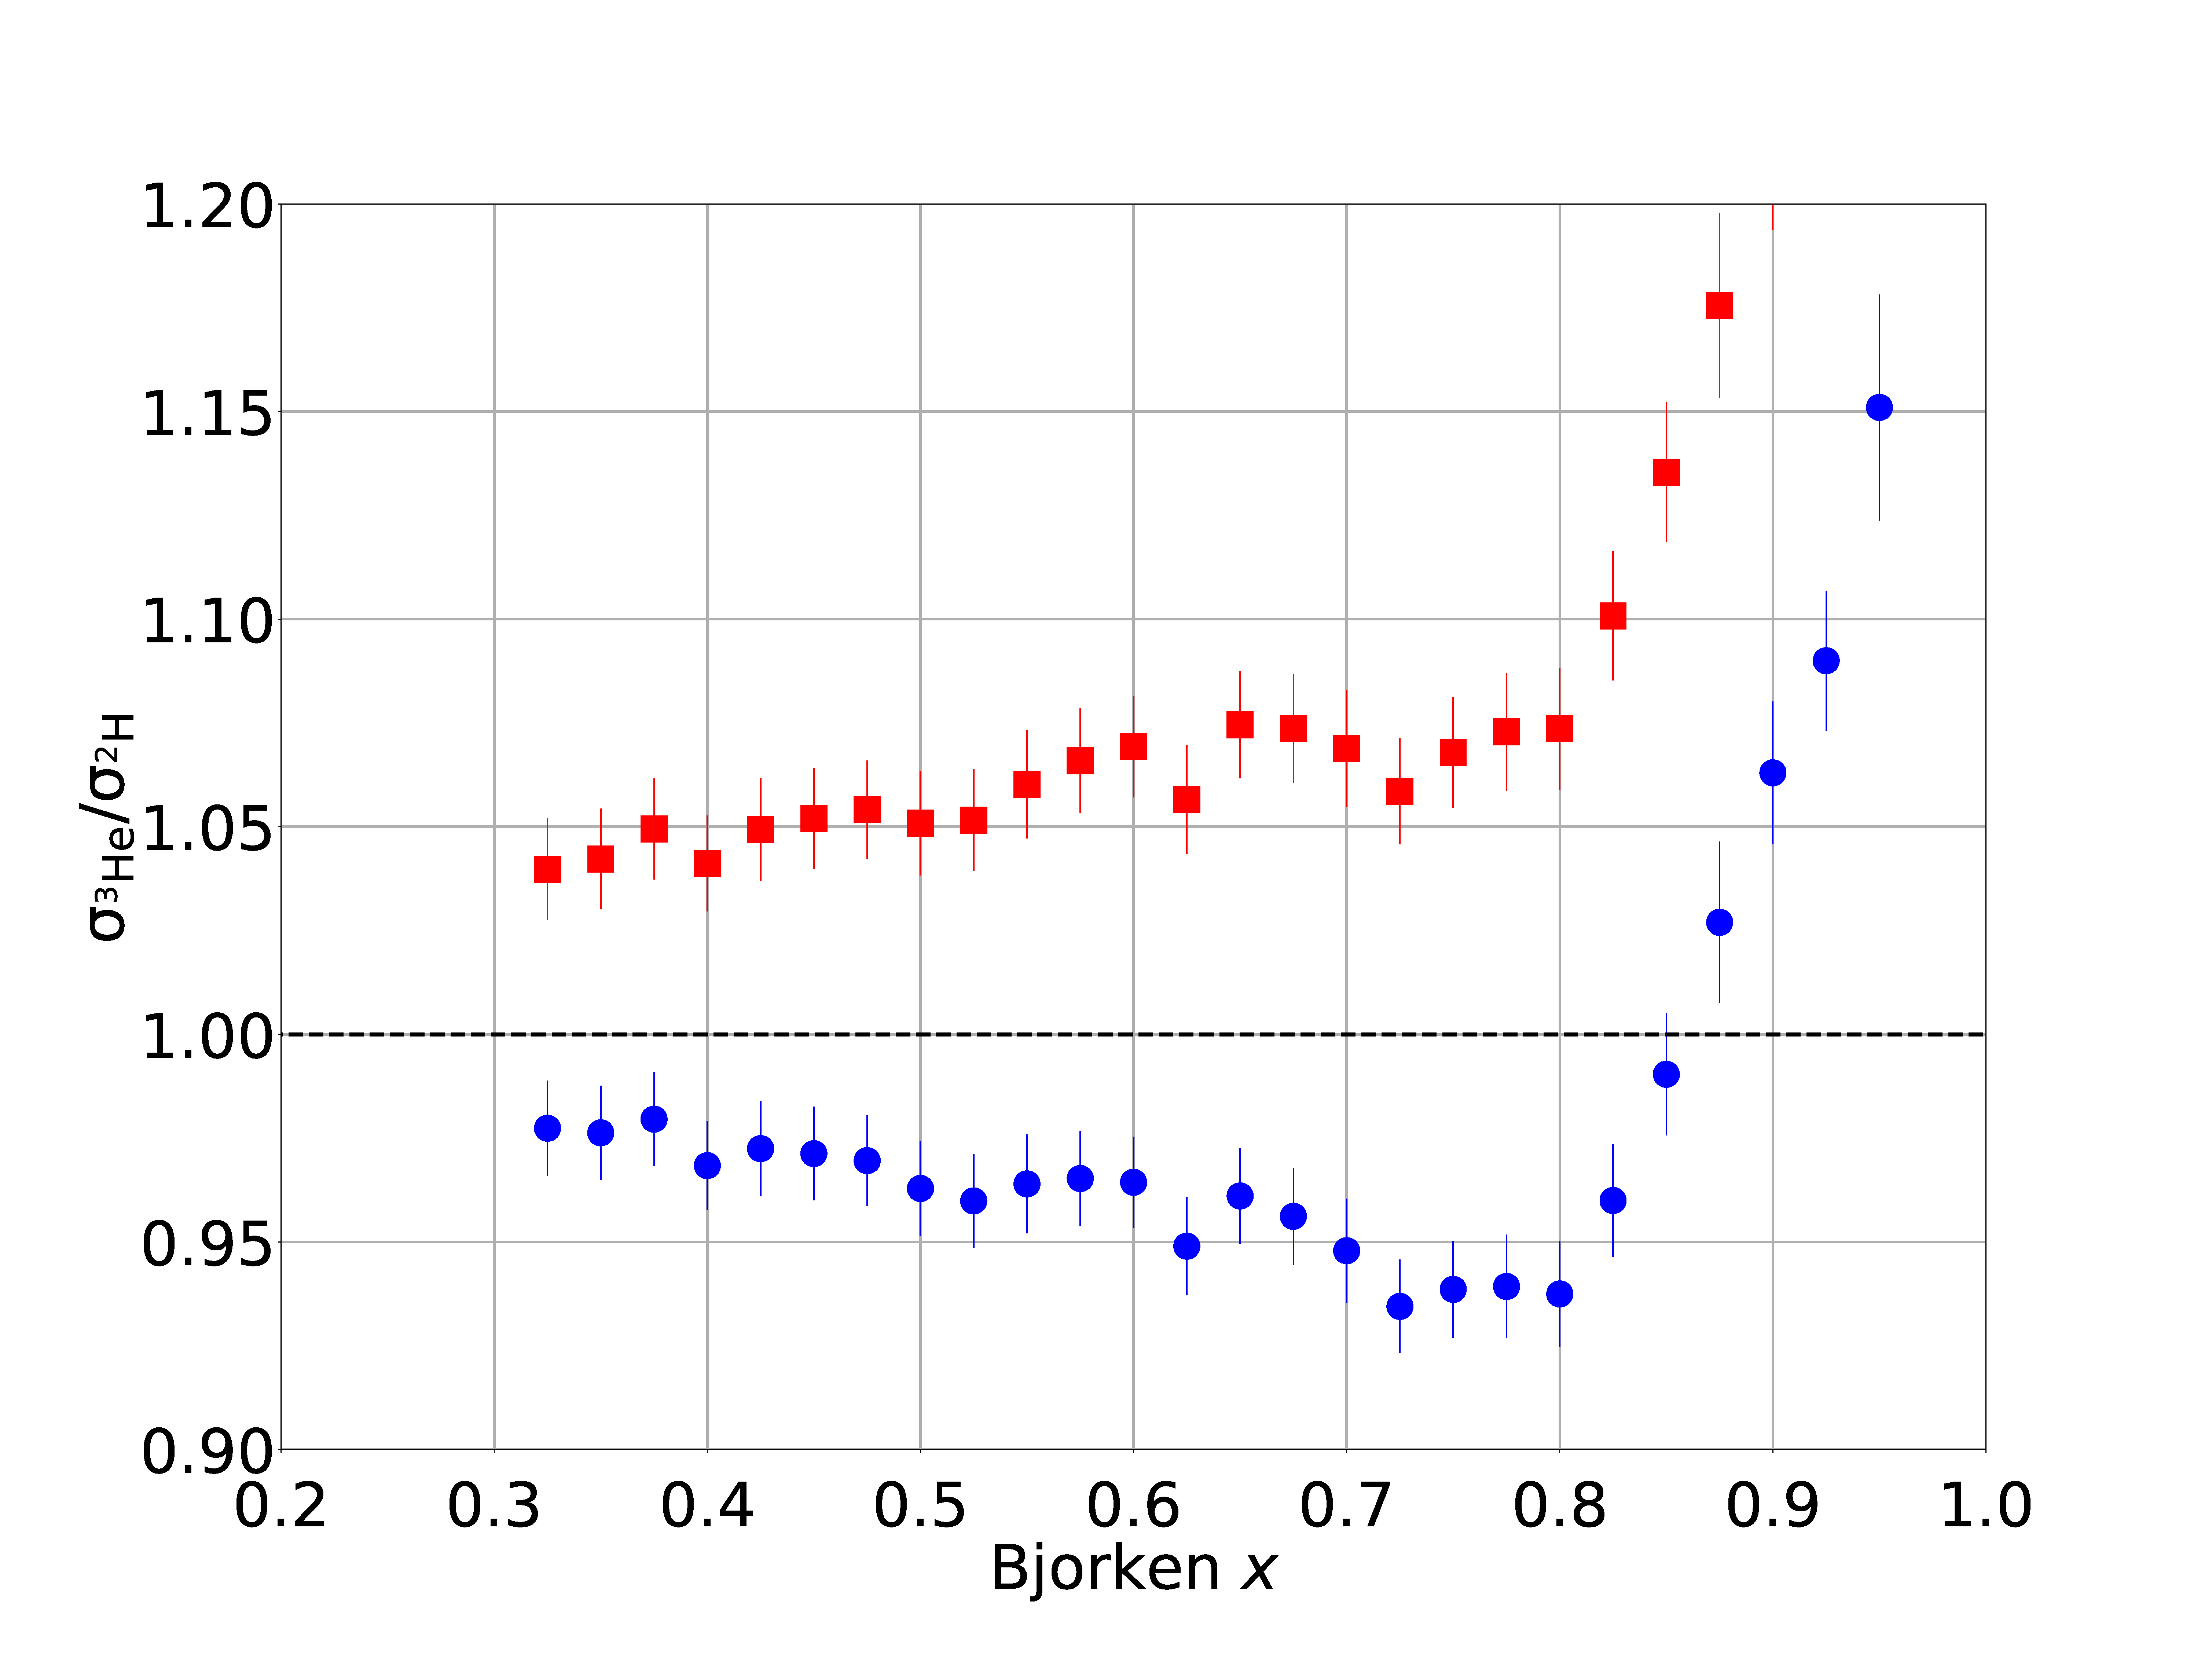
\includegraphics[width=0.7\textwidth]{./EMC/fig/seely.eps}
	\caption{Helium-3 results from JLab E03-103. The upper red squares are the raw ratio and the lower blue circles have an isoscalar correction applied.\cite{e03103}}
	\label{seely_3he}
\end{center}
\end{figure}

\section{Structure Regions}
In DIS $F_2$ structure function data, there are four phenomenological regions. In each region, different physics dominates the shape of the structure function ratio. Each kinematic region provides is a test bed for our understanding of nuclear physics. Studying these nuclear effects is the driving force behind many experiments.

\subsection{Shadowing}

Nuclear shadowing is a phenomenon that occurs in the region of $x<0.1$. Here, there is a depletion of the structure function when compared to deuterium. This depletion increases with mass number $A$. This depletion is also weakly dependent on $Q^2$ and mass number A. This effect is typically explained in terms of nuclear scattering which can be further investigated in reference \cite{shadowing}.
%at roughly the $\ln Q^2$ scale.

\subsection{Anti-shadowing}

The Anti-shadowing, or enhancement, region is from $0.1 \leq x \leq 0.3$. In this region, the EMC structure function ratios are enhanced to greater than 1. Within experimental uncertainties, there is no $Q^2$ dependence in the anti-shadowing region.

\subsection{EMC Effect}

The EMC Effect region spans from $0.3 \leq x \leq 0.8$. In this kinematic area, the EMC structure function ratio falls off and reaches a minimum around $x=0.65$. Since the discovery of the effect by the European Muon Collaboration, extensive EMC Effect region data has been recorded over a large $Q^2$ range. The data suggests that the EMC Effect is largely independent of $Q^2$. The EMC Effect does appear to be logarithmically dependent on mass number A.

\subsection{Fermi Motion}

As $x$ is pushed past $0.8$ the EMC structure function ratio sharply increases far beyond unity. In this region it is known that $F_2^N$, the free nucleon structure function, to drop as $\left(1-x\right)^3$. Fermi motion increases the structure function of the bound nucleon, causing the ratio to show this sharp increase.

\section{Theories}
There are many theories as to the origin of the EMC effect. To cover them all is beyond the scope of this thesis; however, this section will discuss the broad classes of models which can be investigated further in \cite{Norton,GST,HenSRC}.

There are two primary groups of theories. Nuclear Structure focuses on the physics of scattering from a nucleus. Nucleon modification focuses on changes to quark momenta due to confinement effects.

\subsection{Nuclear Structure}

\subsubsection{Nucleon Models}

Traditional scattering calculations assume that the scattered nucleon was on-shell. This class of models gives the struck nucleon an average separation energy $\left\langle\epsilon\right\rangle$, resulting in a shift of its average energy. The inclusion of this term moves the nucleon off-shell. This energy shift causes a rescaling of the $x$. This rescaling can explain the EMC effect region and Fermi motion. However, it is not capable of reproducing the anti-shadowing region.

\subsubsection{Pion Enhancement}

Pion Enhancement models describe an enhancement of the nuclear pion field by nucleon-nucleon interactions. In these models the pion contribution is concentrated to low $x$. The creation of pions also requires the creation of $\Delta$ resonances in the nucleus. 

Alone, this class of model has several problems. To reproduce high $x$ data requires the presence of significantly more $\Delta$s than calculations suggest are plausible. In addition to this, matching anti-shadowing data causes a mismatch in high $x$ data.

\subsection{Nucleon Modification}

\subsubsection{Quark Bags}

In quark cluster models, quarks are confined to ``bags'' as defined by the MIT bag model. This creates color-singlet states with multiples of 3 quarks. The most common quark bag models rely on 6-quark bags. 6-quark bags are larger than a nucleon and thus lead to partial deconfinement of the quarks. This increase in confinement size leads to a decrease in quark momenta due to the uncertainty principle. A decrease in quark momenta in this way will suppress the structure function in the EMC region, leading to the EMC effect \cite{Norton,HenSRC}.

This quark bag model alone can compute many nuclear affects. It is hampered by the need for an additional free parameter to compute each new observable. This model has fallen out of favor due to failed predictions in the nuclear Drell-Yan process \cite{HenSRC}.

\subsubsection{Mean Field Enhancement}

Mean Field Enhancement suggests that the structure functions of the nucleons are modified by nucleus surrounding them. Nucleons confined within the nucleus exchange mesons between the quarks of other confined nucleons. This modifies the structure of the nucleon to change the size of the quark confinement. The predicted increase in confinement size yields a smaller quark momentum \cite{HenSRC,Daniel_thesis}.

\subsubsection{Short Range Correlations}

Short-Range Correlations (SRCs) greatly modify a few nucleons, rather than the small modification to all nucleons in mean-field enhancement. SRCs are the idea that there is a probability that two nucleon wavefunctions will overlap. In this scenario, the overlapping wavefunctions will cause the size of quark confinement within the correlated nucleons to greatly increase, drastically decreasing the quark momenta.

SRCs also predict an observed high momentum tail at $x>1$. Studies of this effect have noted a correlation between the SRC ``scale factor'' and the strength of the EMC effect, the slope of the EMC ratio in the EMC region \cite{HenSRC,CLASSRC,WeinsteinSRC}.

\subsubsection{Discerning between Mean Field Enhancement and SRCs}

Both Mean Field Enhancement and SRCs have been shown to have accurate predictive power within the datasets available. This leads to the conundrum of finding an unmeasured quantity for which the two models make different predictions. Hen \cite{HenSRC} and Thomas \cite{ThomasSRC} discuss that mean field theory and SRCs make seemingly contradictory predictions for the polarized EMC effect. Mean field enhancement predicts that polarization will enhance the effect; SRCs predict the polarization to minimize the effect. This will be tested in Jefferson Lab Hall B with the CLAS spectrometer by measuring the spin structure functions of $^7$Li \cite{CLASspinEMC}.

%\subsection{First subsection}
%
%This is the first subsection of the first section of the first Chapter....
%
%
%\begin{table}[ht]
%\caption{Quarks, Leptons and Gauge Bosons}			% title of Table
%\centering										% used for centering table
%\begin{tabular}{l c c c r}							% centered columns (5 columns)
%\hline										%inserts single horizontal line
%Generation		& Quark 						& Electric Charge($\left | q_{e} \right |$)	& Mass($MeV/c^{2}$)	& Spin\\ 	 	% inserts table
%\hline										% inserts single horizontal line
%First				&Up (u)						& +2/3							& 1.7-3.1				& 1/2\\	%insertingbodyofthetable
%				& Down (d)					& -1/3							& 4.1-5.7				& 1/2\\[1ex]
%Second			& Charm (c)					& +2/3							& 1180-1340			& 1/2 \\
%				& Strange (s)					& -1/3 							& 80-130				& 1/2 \\[1ex]
%Third				& Top (t)						& +2/3 							& 172900$\pm$1500	& 1/2 \\
%				& Bottom (b) 					& -1/3		 					& 4130-4370			& 1/2 \\ [1ex]% [1ex] adds vertical space 
%\hline
%Generation		& Lepton						& Electric Charge($\left | q_{e} \right |$)	& Mass($MeV/c^{2}$)	& Spin\\ 
%\hline
%First				& Electron (e)					& -1								& 0.511				& 1/2\\
%				& Electron Neutrino ($\nu_{e}$)	& 0								& 0					& 1/2\\[1ex]
%Second			& Muon ($\mu$)				& -1								& 105.66				& 1/2\\
%				& Muon Neutrino ($\nu_{\mu}$)	& 0								& 0					& 1/2\\[1ex]
%Third				& Tau ($\tau$)					& -1								& 1776.84				& 1/2\\
%				& Tau Neutrino ($\nu_{\tau}$)		& 0								& 0					& 1/2\\[1ex]
%\end{tabular}
%\begin{tabular}{c c c c c}
%\hline
%Force			& Gauge Boson				& Electric Charge($\left | q_{e} \right |$)	& Mass($GeV/c^{2}$)	& Spin\\ 
%\hline
%Electromagnetic	& $\gamma$ (Photon)			& 0								& 0					& 1\\[1ex]
%Weak Nuclear		& $W^{\pm}$					& $\pm 1$							& 80.3980$\pm$0.025	& 1\\
%				& $Z^{0}$						& 0								& 91.1876$\pm$0.0021	& 1\\[1ex]
%Strong Nuclear		& g (8 Gluons)					& 0								& 0					& 1\\[1ex]
%\hline
%\end{tabular}
%\label{table:nonlin}								% is used to refer this table in the text
%\end{table}
%
%\newpage 
%
%
%\subsection{Second subsection}
%
%This is the second subsection....
%
%Here comes a Figure......
%
% \begin{figure}[!htbp]
%  \begin{center}
%    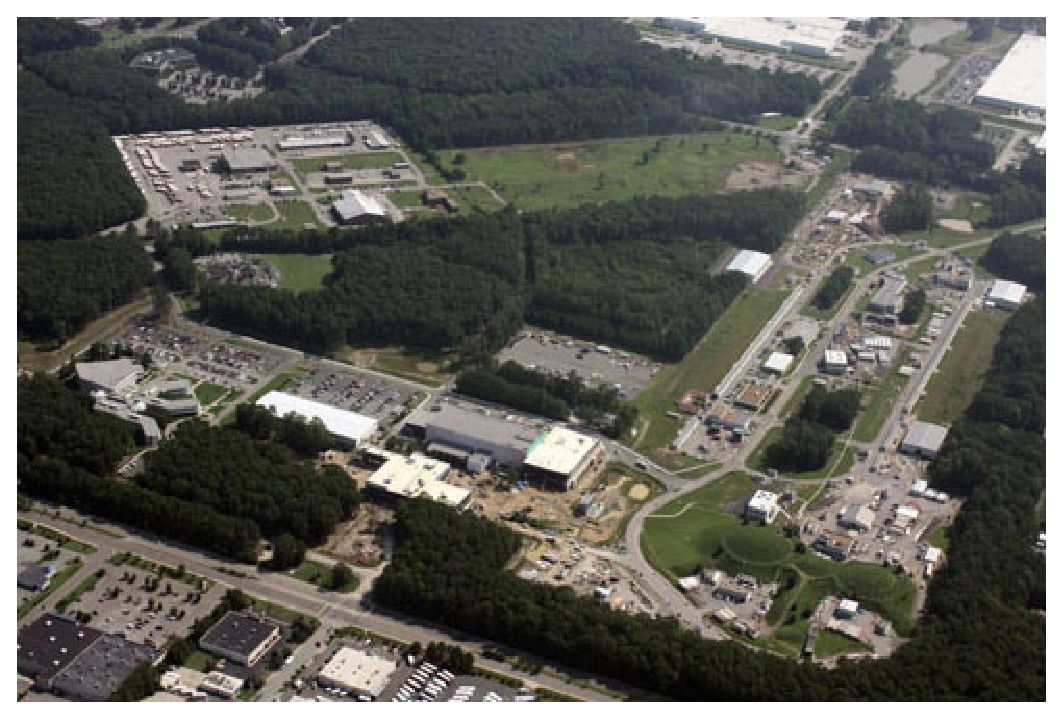
\includegraphics[angle=0, scale=0.85]{./chap1-intro/fig/Visit-JLab3.eps}
%  \end{center}
%  \caption[Aerial view of Jefferson Laboratory, Newport News, Virginia.]{
%    \footnotesize Aerial view of JLab
%  }
%  \label{fig:AerJLab}
%\end{figure}
%
%
%
%Use the label name to refer to  Figure  ~\ref{fig:AerJLab}.
%
%\subsubsection{Sub sub section a}
%
%This is a subsubsection
%
%\subsubsection {Sub sub section b}
%
%Another subsubsection......

